\documentclass{article}
\usepackage{pgfplots}
\pgfplotsset{compat=1.17} % Adjust the version number as needed

\begin{document}

\begin{figure}[h]
    \centering
    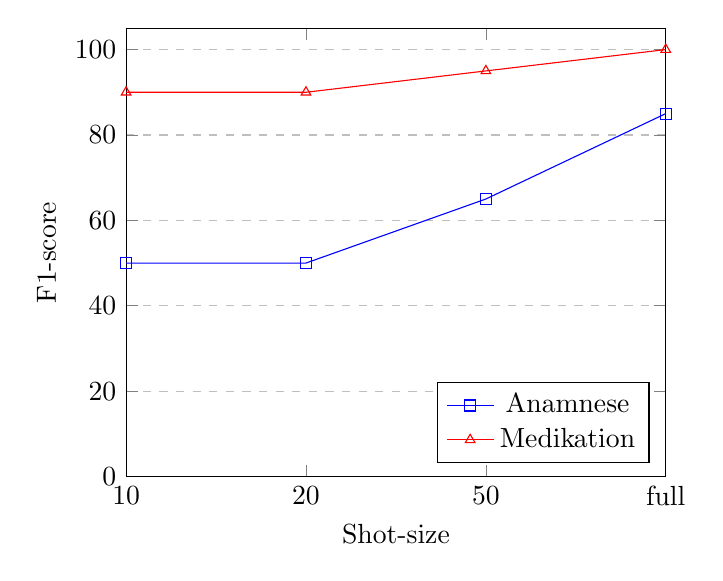
\begin{tikzpicture}
        \begin{axis}[
            xlabel={Shot-size},
            ylabel={F1-score},
            xmin=0, xmax=6,
            ymin=0, ymax=105,
            xtick={0,2,4,6},
            xticklabels={10, 20, 50, full},
            ytick={0,20,40,60,80,100},
            legend pos=south east,
            ymajorgrids=true,
            grid style=dashed,
        ]
            \addplot[
                color=blue,
                mark=square,
                ]
                coordinates {
                    (0,50) (2,50) (4,65) (6,85)
                };
            \addplot[
                color=red,
                mark=triangle,
                ]
                coordinates {
                    (0,90) (2,90) (4,95) (6,100)
                };
            \legend{Anamnese, Medikation}
        \end{axis}
    \end{tikzpicture}
    \caption{\textbf{Core experiments: Primary class F1-score for all shot sizes}. $F1$-score per few-shot sizes for primary classes with no context using \textit{gbert-base-comb nocontext}.}
    \label{fig:core_experiments_f1_score}
\end{figure}

\end{document}